\documentclass[dvipdfmx,fleqn]{beamer}
%\documentclass[dvipdfmx,fleqn,handout]{beamer}
\usepackage{amsmath,amssymb,amsthm,pxjahyper}
\usepackage{minijs}
\usepackage{otf}
\mode<presentation>
{
  \usetheme{Hannover}
}
\usefonttheme{professionalfonts}
\setbeamertemplate{frametitle}[default][center]
\setbeamertemplate{navigation symbols}{}
\setbeamercovered{transparent}
\setbeamertemplate{footline}[page number]
\setbeamerfont{footline}{size=\scriptsize}

\title{Fictitious Play by Python}
\author{Naoya Sho}
\institute{Oyama Seminar, University of Tokyo}
\date{28 Jun 2014}

\sffamily
\gtfamily

\begin{document}
\begin{frame}\frametitle{}
 \maketitle
\end{frame}

\section*{Contents}
\begin{frame}\frametitle{Today's contents}
 \tableofcontents
\end{frame}

\setcounter{framenumber}{0}

\section{Fictitious Play}
\begin{frame}
\frametitle{Fictitious Play}
\begin{itemize}\setlength{\parskip}{0.5em}
\item
A dynamic learning rule where each players rationally behaves based on the belief for the opponents' strategy.
\item
At $t$ round, each player presumes that the opponents follows \textsl{the empirical frequency of strategies} from round $1$ to $t-1$

\item
The learning process can be replicated by programming. In this excersise, two types of games below are covered.

 \begin{itemize}\setlength{\parskip}{0.5em}
 \item
 Matching Pennies
 \item
 $2\times2$ coordination game
 \end{itemize}

\end{itemize}
\end{frame}

\begin{frame}
\frametitle{Fictitious Play in a case of 2 players}
\begin{itemize}\setlength{\parskip}{0.5em}
\item
Diffrence equation of the belief

$x_0(t)$ can be recursively written as
\[
x_0(t+1)
= x_0(t) + \frac{1}{t+2} (a_1(t) - x_0(t))
\]
where $x_0(t)$ is the player 0's belief about the player 1's behavior at time $t$ and $a_1(t)$ is the player 1's action at time $t$.

\end{itemize}
\end{frame}

\section{General Settings}

\begin{frame}
\frametitle{Basic Algorithm}
\begin{itemize}\setlength{\parskip}{0.5em}
\item
A payoff of all the players is given in the form of a matrix.

\item
Buid a best responce function which
 \begin{itemize}\setlength{\parskip}{0.5em}
 \item
 takes the payoff matrix and belief about the opponent's action as inputs

 \item
 returns the action that maximize the expected payoff as an output
 \end{itemize}
\item
For $t = 0, 1, 2...$, iteratively compute each player's action and belief and make a list of belief over the whole procedure.

\end{itemize}
\end{frame}

\begin{frame}
\frametitle{Example games}
\begin{itemize}\setlength{\parskip}{0.5em}
\item
One example of Matching Pennies game is defined as below:

 \begin{table}
 \begin{tabular}{|c|c|c|} \hline
      & Action 0 & Action 1 \\ \hline 
    Action 0 & $1,-1$ & $-1,1$ \\ \hline
    Action 1 & $-1,1$ & $1,-1$ \\ \hline
   \end{tabular}
  \end{table}

\item
One example of $2\times2$ coordination game is defined as below:

 \begin{table}
 \begin{tabular}{|c|c|c|} \hline
      & Action 0 & Action 1 \\ \hline 
    Action 0 & $4, 4$ & $0, 3$ \\ \hline
    Action 1 & $3, 0$ & $2, 2$ \\ \hline
   \end{tabular}
  \end{table}

\item
Note that $2\times2$ coordination game is a symmetric game, where each player has the same payoff structure.

\end{itemize}
\end{frame}

\section{Programming codes}
\begin{frame}[fragile]
\frametitle{Programming codes 1}
\begin{itemize}\setlength{\parskip}{0.5em}
\item
Extracted codes for Matching Pennies game with brief comments
\scriptsize
\begin{verbatim}
pay = ((1,-1),(-1,1),
       (-1,1),(1,-1)) 

def sep(p, pay):
    return ((pay[0][a], pay[1][a]),
            (pay[2][a], pay[3][a]))

\end{verbatim}
\normalsize

\item
First, input the payoff structure in the form of matrix called \texttt{pay}
\item
Then set up the function \texttt{sep(a, pay)}, which
 \begin{itemize}\setlength{\parskip}{0.5em}
 \item
 takes the index of the player and payoff matrix as inputs
 \item
 returns the each player's individual payoff matrix dropping the opponent's payoff. (For later use.)
 \end{itemize}

\end{itemize}
\end{frame}


\begin{frame}[fragile]
\frametitle{Programming codes 2}
\begin{itemize}\setlength{\parskip}{0.5em}
\item
Construct the best responce function.
\scriptsize
\begin{verbatim}
xmat = np.empty((len(players), len(players)))

def br(p,x):
    xmat[p] = (1-x, x)
    expay = np.dot(np.array(sep(p, pay)), xmat[p])

    if expay[0] == expay[1]:
        return random.randint(0,1)

    else:
        return expay.argmax()
\end{verbatim}
\normalsize

\item
p indicates pth player and x denotes his belief about the opponent's action. xmat is a empty $2\times2$ matrix where pth row  has player p's expectation for opponent's each action.

\item
\texttt{expay} is a vector obtained by calculating the product of player p's individual payoff matrix and belief vector.

\item
Finally, returns the biggest element of \texttt{expay} if there is only one (Not very general).
\end{itemize}
\end{frame}


\begin{frame}[fragile]
\frametitle{Programming codes 3}
\begin{itemize}\setlength{\parskip}{0.5em}
\item
Compute the games iteratively.
\scriptsize
\begin{verbatim}
def playgame(trials):

    x0 = random.uniform(0,1)
    x1 = random.uniform(0,1)

    for i in range(1000):
        a0 = br(0, x0)
        a1 = br(1, x1)
        x0.append(x[i]+(a[1]-x[i])/(i+2))
        x1.append(x[i]+(a[0]-x[i])/(i+2))
\end{verbatim}
\normalsize

\item
Here, I used a function so that I can easily try different number of trials.
\item
Choose the action utilizing \texttt{br(p, x)} and put it into the difference equation.

\item
This part can be neatly incoporated by using \texttt{for} loop for each player. (but I gave up)

\end{itemize}
\end{frame}


\section{Graphical outcome}
\begin{frame}
\frametitle{Matching Pennies: Transition of belief}
\begin{figure}
 \centering
 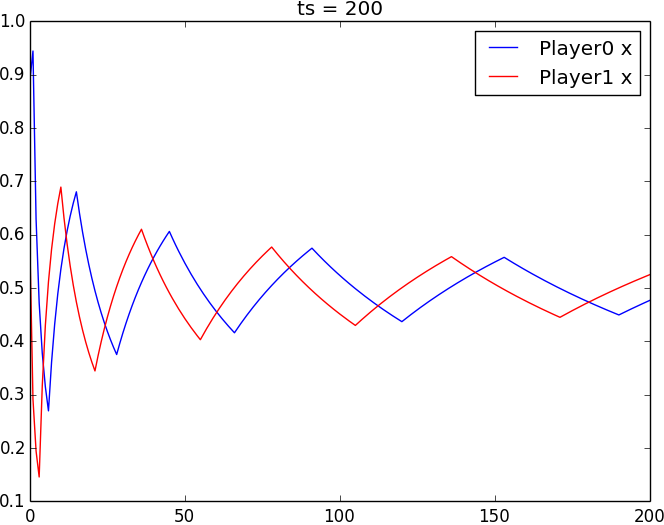
\includegraphics[width=0.7\linewidth]{Matpenny200.pdf}
 \caption{Transition of belife in Matching Pennis game for 200 times}
 \label{fig:Matpenny200}
\end{figure}
\end{frame}

\begin{frame}
\frametitle{Matching Pennies: Histogram of the terminal belief}
\begin{figure}
 \centering
 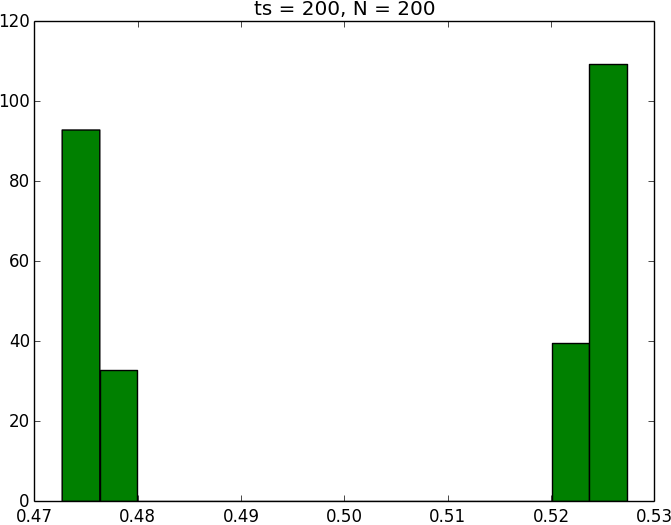
\includegraphics[width=0.7\linewidth]{Matpenny_hist200_200.pdf}
 \caption{200 iterations of Matching Pennis game for 200 times}
 \label{fig:Matpenny_hist200_200}
\end{figure}
\end{frame}


\begin{frame}
\frametitle{$2\times2$ coordination game: Transition of belief pattern 1}
\begin{figure}
 \centering
 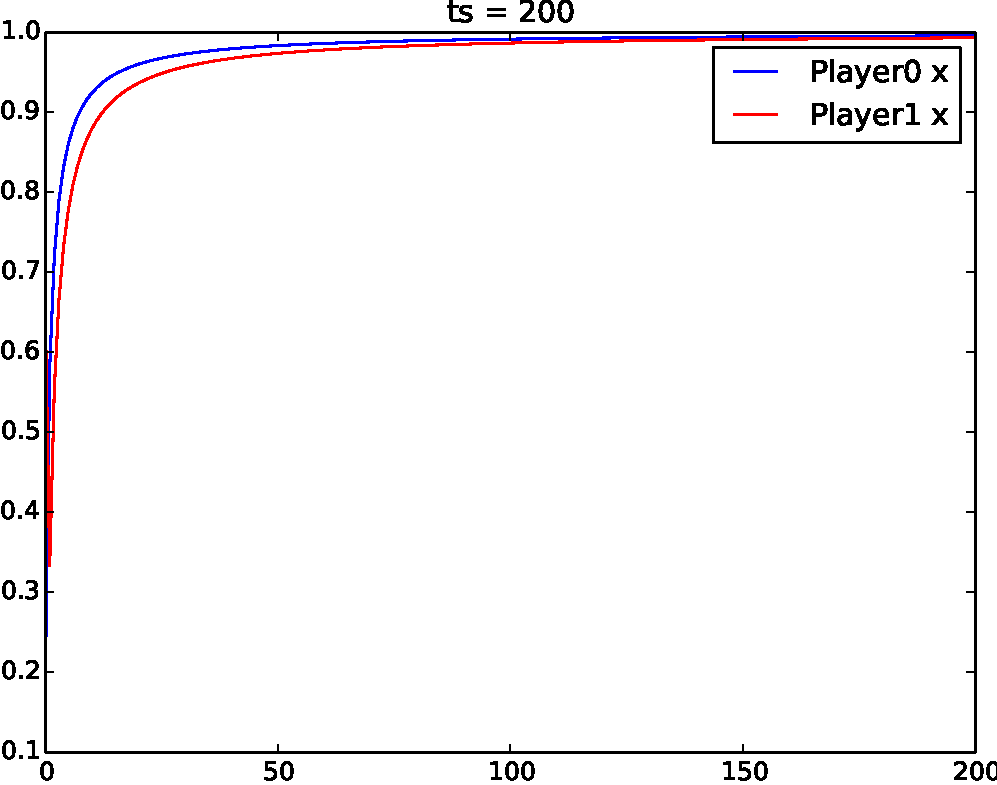
\includegraphics[width=0.7\linewidth]{2coordgame200_1.pdf}
 \caption{$2\times2$ coordination game for 200 times}
 \label{fig:2coordgame200_1.pdf}
\end{figure}
\end{frame}


\begin{frame}
\frametitle{$2\times2$ coordination game: Transition of belief pattern 2}
\begin{figure}
 \centering
 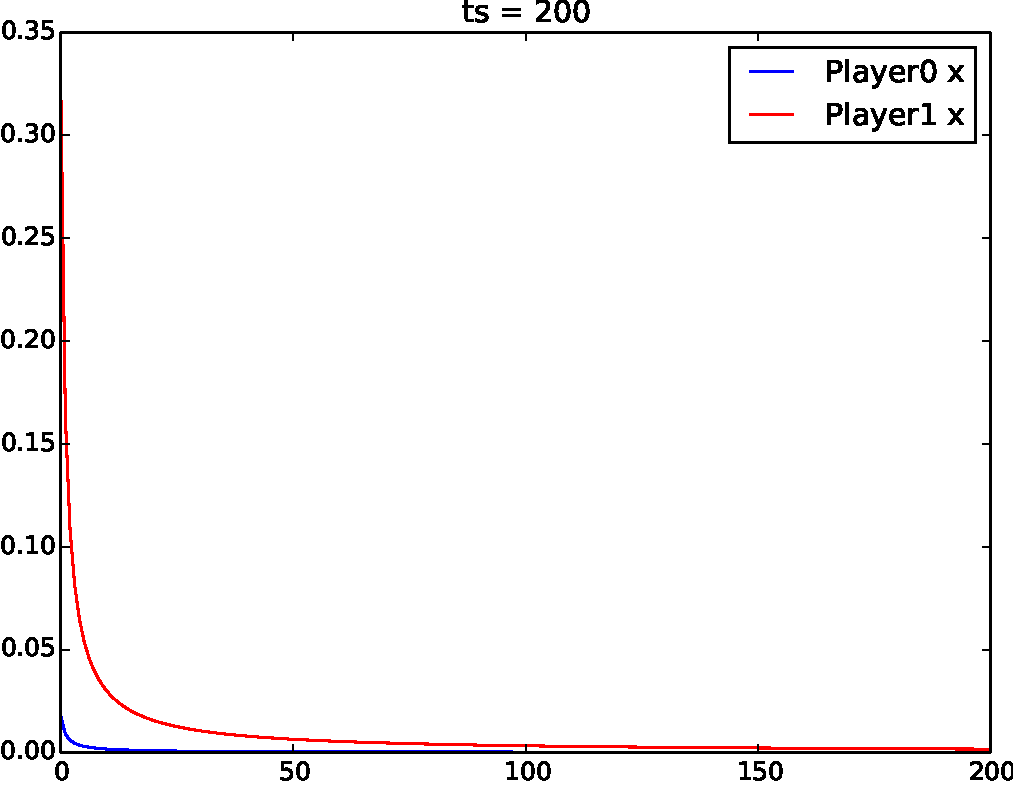
\includegraphics[width=0.7\linewidth]{2coordgame200_2.pdf}
 \caption{$2\times2$ coordination game for 200 times}
 \label{fig:2coordgame200_2}
\end{figure}
\end{frame}


\begin{frame}
\frametitle{$2\times2$ coordination game: Histogram of the terminal belief}
\begin{figure}
 \centering
 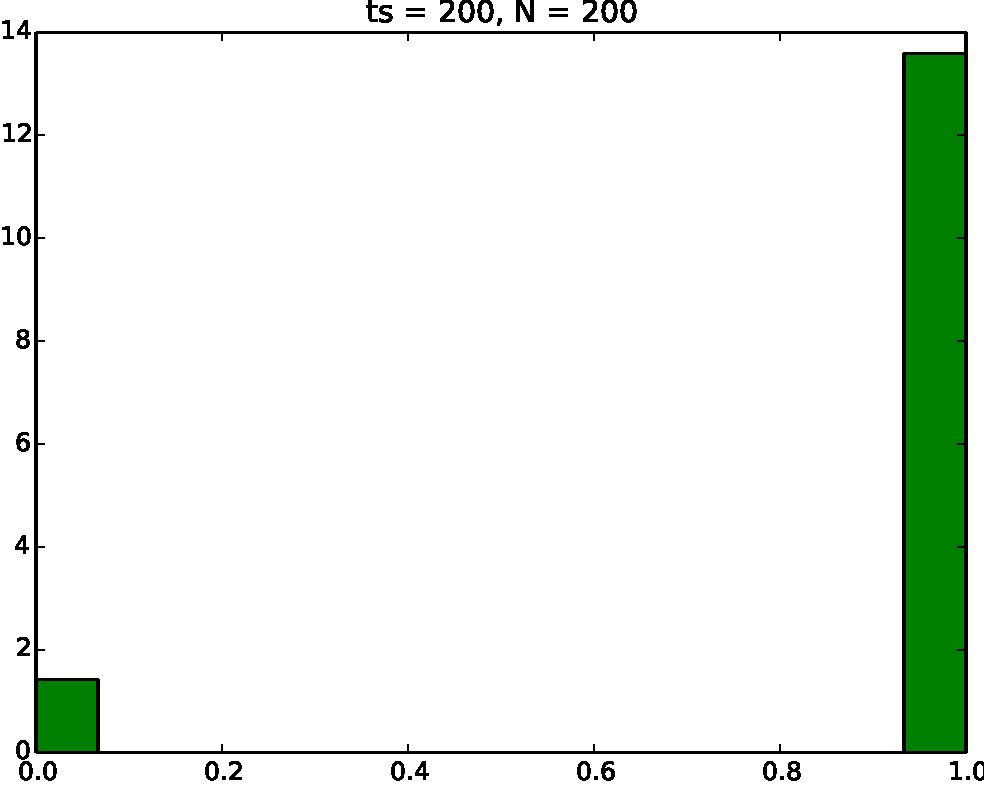
\includegraphics[width=0.7\linewidth]{2coordgame_hist200_200.pdf}
 \caption{200 iterations of $2\times2$ coordination game for 200 times}
 \label{fig:2coordgame_hist200_200}
\end{figure}
\end{frame}


\section{For further improvements}
\begin{frame}
\frametitle{For further improvements}
\begin{itemize}\setlength{\parskip}{0.5em}
\item
OOP can be introduced. I intentionally often used functions so that the transition is smooth. (But not tried yet.)

\item
Introducing \texttt{for} loop for players is a bit clumsy. In the loop for p, I sometimes have to use p as a index for matrices, so end up with messy codes with tons of indexed matrices and vectors. 

\end{itemize}
\end{frame}


\end{document}